\documentclass[12pt]{article}
\usepackage[]{geometry}
\usepackage{titlesec}
\usepackage{enumitem}
\usepackage{tabularx}
\usepackage{color, hyperref, xcolor}
\usepackage[document]{ragged2e}
% \usepackage{fontspec}
\usepackage{xtab}
\usepackage{graphicx}
\usepackage{tabularx}
\usepackage{multirow}
\usepackage{hyperref}

\thispagestyle{empty}
\geometry{paperheight=11.5in, paperwidth=8.5in, margin=0.8cm}
\newcommand{\resumename}[1]{\LARGE\textbf{#1} \hfill \small}
\titleformat{\section} 
  {\normalfont\fontsize{12pt}{10}\bfseries}{\thesection}{1em}{}[{\titlerule[0.8pt]}]
\titlespacing*{\section}{0em}{0.9em}{0.5em}
\titleformat{\subsection}[runin]{\bfseries}{}{}{}[]
\titlespacing*{\subsection}{0em}{0.5em}{0em}
\begin{document}
\noindent
\resumename{Harsh Bang} 



\begin{table}[h]
	\centering
	\begin{tabular}{@{}p{0.8\linewidth}c@{}}
		\begin{tabular}{@{}llll@{}}
			Linkedin & \href{https://www.linkedin.com/in/harsh-bang-696339221/}{linkedin.com/in/harsh-bang-696339221/} &   & Email: \href{mailto:harshbang786@gmail.com}{harshbang786@gmail.com} \\ 
			Codechef & \href{https://www.codechef.com/users/harsh_bang_7}{codechef.com/users/harsh\_bang\_7}               &   & Mobile: \href{tel:+919893649149}{+91-9893649149} \\
			Codeforces & \href{https://codeforces.com/profile/harsh_bang_7}{codeforces.com/profile/harsh\_bang\_7} & & \\
			Github & \href{https://github.com/Harsh9149}{github.com/Harsh9149} & & \\
		\end{tabular} &
		\multirow{4}{*}{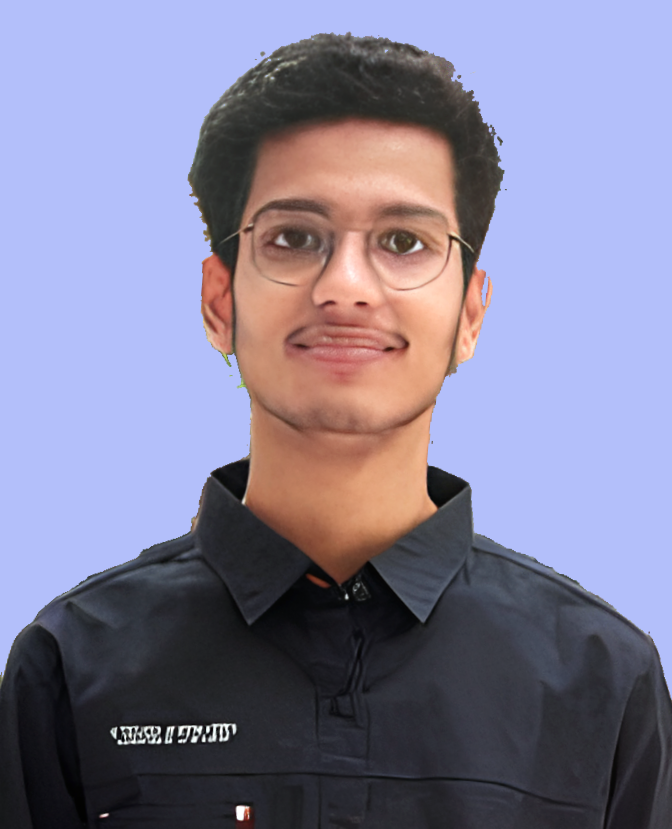
\includegraphics[height=4cm]{passport_photo.png}} \\
	\end{tabular}
\end{table}





% \begin{table}[h]
% 	\centering
% 	\begin{tabularx}{\textwidth}{@{}llXr}
% 		Linkedin & \href{https://www.linkedin.com/in/harsh-bang-696339221/}{linkedin.com/in/harsh-bang-696339221/} &   & Email: \href{mailto:harshbang786@gmail.com}{harshbang786@gmail.com} \\ 
% 		Codechef & \href{https://www.codechef.com/users/harsh_bang_7}{codechef.com/users/harsh\_bang\_7}               &   & Mobile: \href{tel:+919893649149}{+91-9893649149}                                    \\
% 		Codeforces &\href{https://codeforces.com/profile/harsh_bang_7}{codeforces.com/profile/harsh\_bang\_7} \\
% 		Github &\href{https://github.com/Harsh9149}{github.com/Harsh9149} \\
% \end{tabularx}
% \end{table}
\vspace{-\topsep}
\section*{EDUCATION}
\subsection*{Indian Institute of Information Technology, Lucknow}	\hfill\textbf{Lucknow, India} \\
Bachelor of Technology - Information Technology (CGPA: 8.12/10) 	\hfill\textit{December 2020 - Present} \\
\subsection*{Macro Vision Academy}	\hfill\textbf{Burhanpur, Madhya Pradesh, India} \\
CBSE Class XII (Percentage: 91.4) \hfill \textit{2020} \\
\subsection*{Narmada Valley International School}	\hfill\textbf{Barwaha, Madhya Pradesh, India} \\
CBSE Class X (Percentage: 85.6) \hfill \textit{2018} \\

\section*{EXPERIENCE}
\textbf{Codenation - SDE Intern} \hfill \textit{May 2023 - Present (July 2023)} \\
Remote \\

\section*{PROJECTS}
\subsection*{Note Manager website} \quad HTML $|$ CSS $|$ JS $|$ NodeJS $|$ PostgreSQL \\
\begin{itemize}[topsep=0pt,itemsep=1pt,partopsep=3.5pt, parsep=1pt]
	\item A web-based project that helps manage notes privately and securely.
	\item Register securely, view previous notes, and create, update, and delete notes.
	\item Used HTML, CSS, JS for the frontend and NodeJS for the backend with PostgreSQL database.
	\item \textbf{Project Link:} \href{https://github.com/harsh_bang/Note-Manager}{github.com/harsh\_bang/Note-Manager}
\end{itemize}
\subsection*{{StoryTellers}}~ Django $\vert$ Data Structures $\vert$ CSS $\vert$ JavaScript $\vert$ Bootstrap \hfill \textit{April 2022 - June 2022} \\
\begin{itemize}[leftmargin=*,topsep=0pt,itemsep=1pt,partopsep=1pt, parsep=1pt]
	\item Developed a Storyteller website using Django, CSS, JavaScript, and Bootstrap 
	\item In this site, there are a lot of books to read as well as there are audio books and we can also create book using ckeditor.
\end{itemize}
\subsection*{{Blogging Site}}~ Django $\vert$ Data Structures $\vert$ CSS $\vert$ JavaScript $\vert$ Bootstrap $\vert$ Web Socket \hfill \textit{April 2022 - June 2022} \\
\begin{itemize}[leftmargin=*,topsep=0pt,itemsep=1pt,partopsep=1pt, parsep=1pt]
	\item Developed a Blogging website using Django, CSS, JavaScript, and Bootstrap 
	\item In this website you will learn about technical fields of future.
You will learn about Competitive Coding,
Machine Learning,
Web development,
App development,
Data Structures and Algorithm
and Artificial Intelligence.
If you have any questions feel free to contact me through the Contact Page.
\end{itemize}
\section*{ACHIEVEMENTS}
\begin{itemize}[leftmargin=*, topsep=1pt, itemsep=1pt, partopsep=1pt, parsep=2pt]
	\item Rated \textbf{Candidate Master} on \href{https://codeforces.com/profile/Harsh_Bang_7}{Codeforces} (Max Rated: \textbf{1986})
	\item Global Rank \textbf{122} in 
\href{https://codeforces.com/contest/1809/standings/2/participant/151861802#p151861802}{Codeforces Educational Round 145 (Div.2)}
	\item Global Rank \textbf{126} in \href{https://codeforces.com/contest/1798/standings/participant/152311755#p152311755}{Codeforces Round 860 (Div.2)}
	\item Rated \textbf{5 star} on \href{https://www.codechef.com/users/harsh_bang_7}{Codechef} (Max Rated: \textbf{2002})
	\item Global Rank \textbf{40} in \href{https://www.codechef.com/rankings/START35B?itemsPerPage=100&order=asc&page=1&search=harsh_bang_7&sortBy=rank}{Codechef Starters 35 (Div.2)}
	\item Global Rank \textbf{53} in \href{https://www.codechef.com/rankings/COOK140B?itemsPerPage=100&order=asc&page=1&search=harsh_bang_7&sortBy=rank}{Codechef April Cook-Off}
	\item Google Kickstart 2022 Round F ranked \textbf{632}
	\item Google Kickstart 2022 Round G ranked \textbf{724}
	\item Google Kickstart 2022 Round H ranked \textbf{915}
\end{itemize}
\section*{TECHNICAL SKILLS}
\begin{tabular}{@{}llll}
	\textbf{Languages}               && C, C++, JavaScript , Python                                              		\\
	\textbf{Developer Tools}         && Git/Github                                               		\\
	\textbf{Technologies}            && Bootstrap, NodeJS, Express, Django, MySQL, LangChain \\
	\textbf{Academic Coursework}     && Data Structures and Algorithms, OOPS, DBMS, Operating System ,Computer Networks                                          \\
	\vspace{-\topsep}
\end{tabular}

\end{document}